\documentclass[dvipdfmx]{article}
\usepackage[dvipdfmx]{graphicx}
\usepackage{amsmath, amssymb}
\usepackage{mathtools}
\usepackage{here}
\usepackage{caption}

\begin{document}
\title{Weekly Report}
\author{Riku Gondow}
\maketitle
\section{Progress}
\begin{itemize}
    \item Continue to work on the implementation of DDLM
    \begin{itemize}
        \item It may take some more time to implement. Therefore, it may be better to give a priority to look for other open sources and compare them with the datasets that were used for DDLM.
    \end{itemize}
    \item Read a paper titled "Identity Authentication in Two-Subject Environments Using Microwave Doppler Radar and Machine Learning Classifiers"[1]
\end{itemize}

\section{Details of the paper[1]}

The main challenge, and thus the focus of this research, is the recognition of closely spaced subjects within the beamwidth of the radar transceiver(=30°).
Two subjects with a similar physique were (otherwise) randomly paired and arranged in a seated position in front of the radar system as shown in Fig.1.

\begin{figure}[H]
\begin{center}
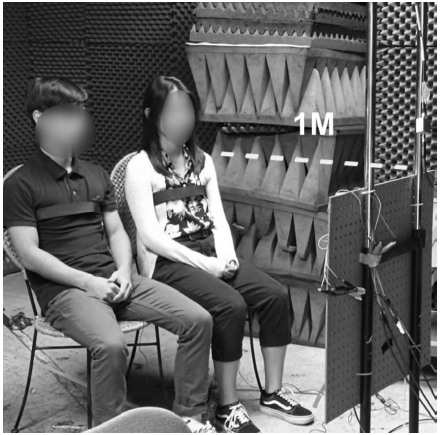
\includegraphics[width=0.55\linewidth]{./img/setting_respi.png}
\end{center}
\caption{Human experiment setup in an anechoic chamber}
\end{figure}

\begin{figure}[H]
\begin{center}
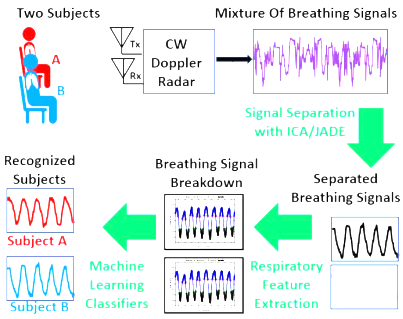
\includegraphics[width=0.85\linewidth]{./img/system_respiration.png}
\end{center}
\caption{Proposed noncontact identity authentication system for two-subject environments}
\end{figure}

In this paper, accuracies of 97.5\% for two-subject experiments and 98.33\% for single-subject experiments were achieved, which supersedes the performance of prior reported methods.

The investigated
features have been classified into two different spaces shown
in Table1. One of them is typical features and another one
is hyperfeatures. The typical respiratory feature extraction
process is described in prior work[2][3].

The extracted hyperfeature sets were then evaluated by integrating two different popular ML classifiers, k-nearest neighbor (KNN) and support vector machine (SVM), for subject authentication.

\begin{figure}[H]
\caption*{Table1: Extracted breathing dynamic-related features}
\begin{center}
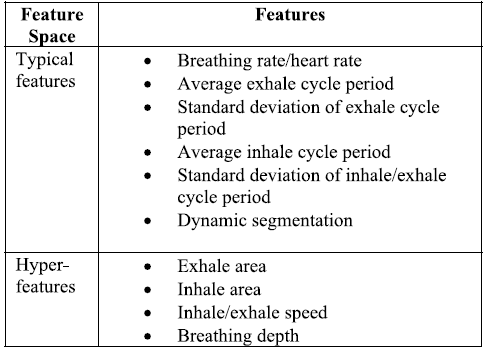
\includegraphics[width=0.8\linewidth]{./img/features_respiration.png}
\end{center}
\end{figure}

\subsection*{Proposed algorithm to determine the inhale and exhale areas, and speed (called hyperfeatures)}
\begin{enumerate}
    \item Preprocessing and separation of respiratory signal using ICA-JADE(: Independent component analysis with the joint approximation of diagonalization of eigenmatrices)
    \item Segmentation of the signal for 12.8 second window
    \item Create an array of local maxima and minima
    \item Grouping of two consecutive maxima and in between one minima for triangulation (as shown in Fig.3)
    \item Calculation of the area of the triangles (inhale and exhale episodes)
    \item Average out the areas (inhale and exhale episodes)
\end{enumerate}

\begin{figure}[H]
\begin{center}
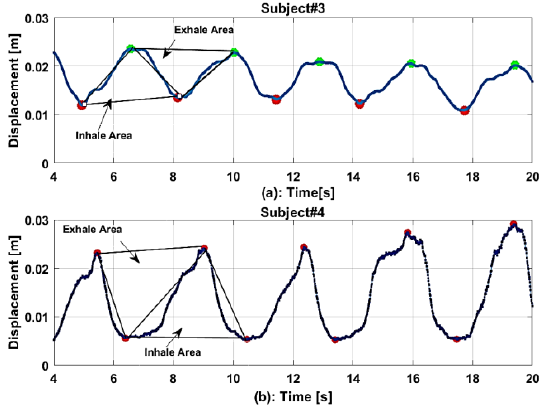
\includegraphics[width=0.8\linewidth]{./img/triangulation.png}
\end{center}
\caption{Illustration of inhale and exhale areas of two subjects}
\end{figure}

\begin{figure}[H]
\caption*{Table2: Accuracy of the different ML classifiers}
\begin{center}
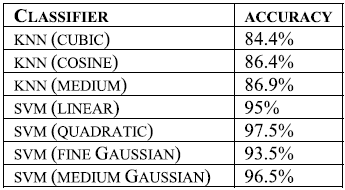
\includegraphics[width=0.8\linewidth]{./img/result_respi.png}
\end{center}
\end{figure}

Among all classifiers, SVM with a quadratic function outperformed the others with an accuracy of 97.5\%.


\begin{figure}[H]
\caption*{Table3: Comparison of this article with other recent relevant works}
\begin{center}
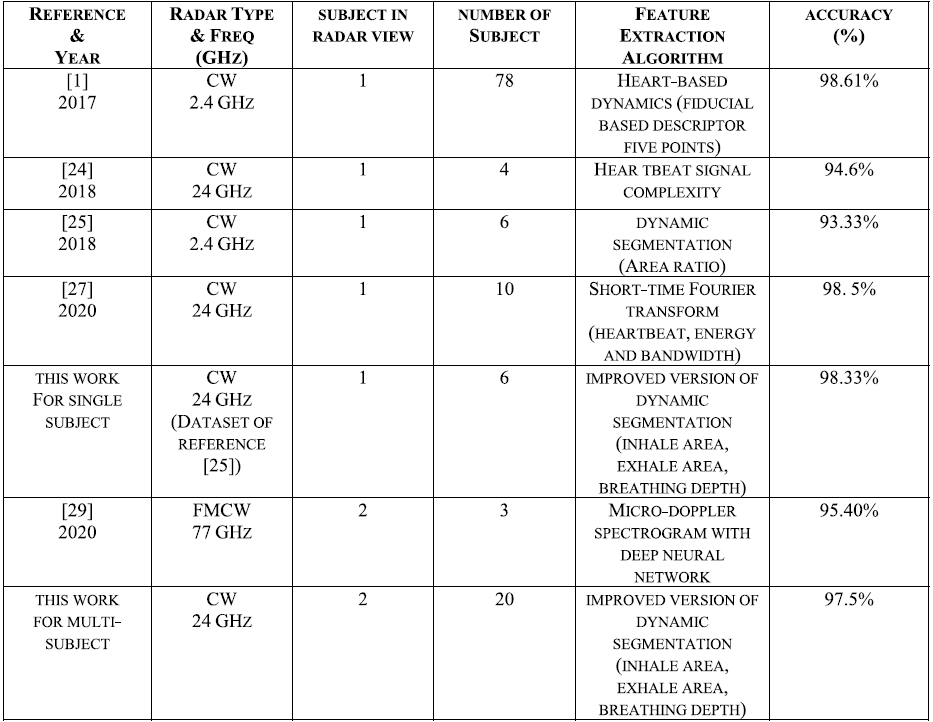
\includegraphics[width=\linewidth]{./img/result_comparison_respi.png}
\end{center}
\end{figure}

The proposed improved dynamics segmentation algorithm with an ML-based approach shows reasonable accuracy compared to the deep learning-based approach.

\section{Next Plan}
\begin{itemize}
    \item Implement DDLM or search open sources to compare accuracy
    \item Consider other approaches
\end{itemize}

\begin{thebibliography}{99}
\bibitem Islam, Shekh MM, Olga Borić-Lubecke, and Victor M. Lubecke. "Identity Authentication in Two-Subject Environments Using Microwave Doppler Radar and Machine Learning Classifiers." IEEE Transactions on Microwave Theory and Techniques (2022).
\bibitem A. Ragman, V. M. Lubecke, O. Boric-Lubecke, J. H. Prins, and
T. Sakamoto, “Doppler radar techniques for accurate respiration characterization
and subject identification,” IEEE J. Emerg. Sel. Topics
Circuits Syst., vol. 8, no. 2, pp. 350–359, Jun. 2018, doi: 10.1109/
JETCAS.2018.2818181.
\bibitem S. M. M. Islam, A. Sylvester, G. Orpilla, and V. M. Lubecke, “Respiratory
feature extraction for radar-based continuous identity authentication,”
in Proc. IEEE Radio Wireless Symp. (RWS), San Antonio, TX,
USA, Jan. 2020, pp. 119–122.
\end{thebibliography}
\end{document}